73. $\cfrac{x^2(x^2-2x+1)}{(x+7)^3(3-x)}\leqslant0\Leftrightarrow\cfrac{x^2(x-1)^2}{(x+7)^3(3-x)}\leqslant0.$\\ Применив метод интервалов, найдём ответ:
\begin{figure}[ht!]
\center{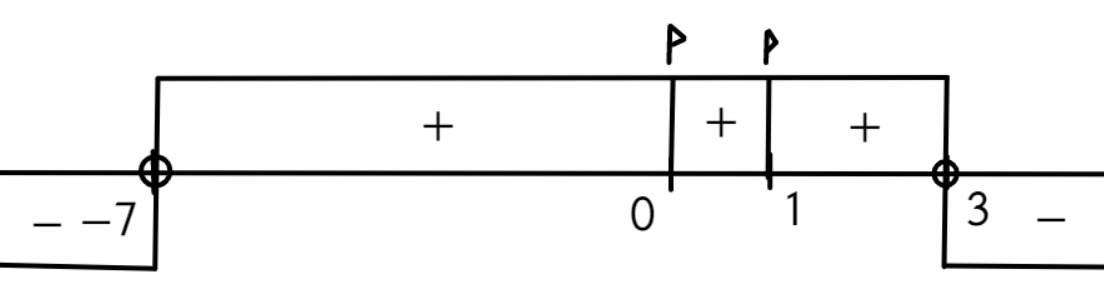
\includegraphics[scale=0.35]{int73.png}}
\end{figure}
$x\in(-\infty;-7)\cup\{0;1\}\cup(3;+\infty).$\\
